\subsection*{Модель разрешения конфликта}
\addcontentsline{toc}{subsection}{Модель разрешения конфликта}

\textbf{Задание:}\\
Провести численный анализ модели разрешения конфликта в среде AnyLogic. Разрешится ли конфликт за 120 дней ?\\

\textbf{Решение:}
\begin{align*}
	\begin{cases}
		\dfrac{dN_1}{dt} = - \alpha_1 (a - N_1) (b - N_2) + \beta_1 N_1 N_2\\[10pt]
		\dfrac{dN_2}{dt} = - \alpha_2 (a - N_1) (b - N_2) + \beta_2 N_1 N_2\\
	\end{cases}
\end{align*}

$N_1(0) = N_{10}$, $N_2(0) = N_{20}$\\
$a = a_0 e^{\frac{n_1 t}{T}}$, $b = b_0 e^{\frac{n_2 t}{T}}$\\
$\alpha_1 = \alpha_{10} e^{\frac{n_3 t}{T}}$, $\alpha_2 = \alpha_{20} e^{\frac{n_4 t}{T}}$\\
$\beta_1 = \beta_{10} e^{\frac{n_5 t}{T}}$, $\beta_2 = \beta_{20} e^{\frac{n_6 t}{T}}$\\

Условие разрешения конфликта:
\begin{align*}
	\begin{cases}
		\dfrac{a}{2} < N_1 \leq a\\[10pt]
		\dfrac{b}{2} < N_2 \leq b\\
	\end{cases}
\end{align*}

В соответствии с формулами, данная модель была реализована в среде моделирования AnyLogic. (Рисунок \ref{fig:conflict1})
\begin{figure}[h]
	\centering 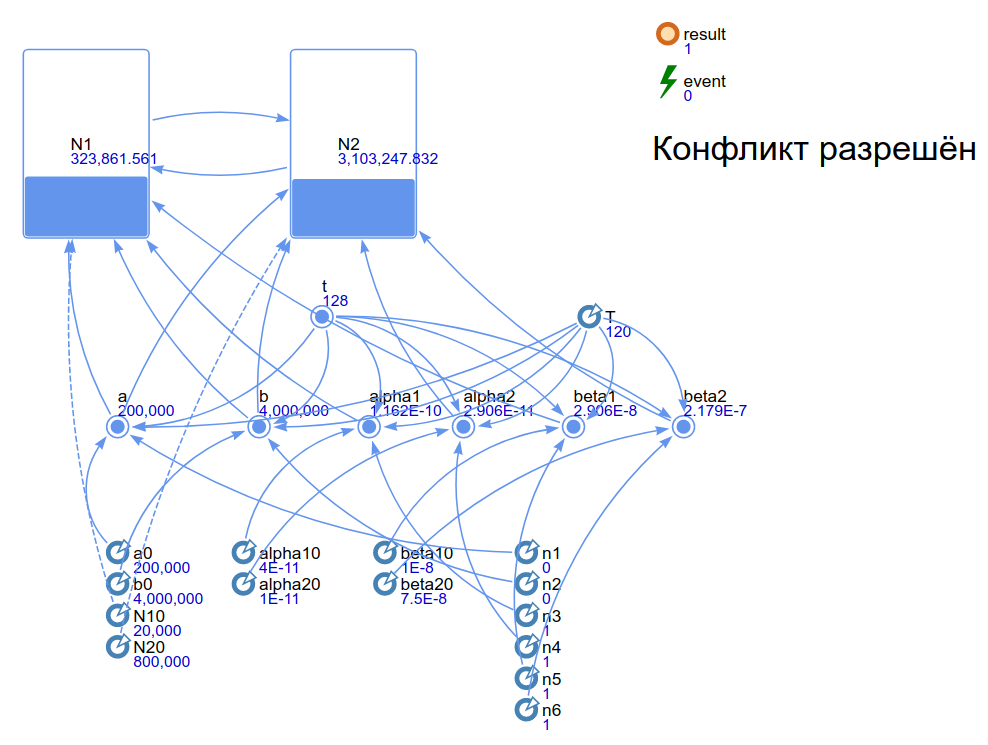
\includegraphics[scale=0.25]{conflict1}
	\caption{Результаты построения модели разрешения конфликта в AnyLogic}
	\label{fig:conflict1}
\end{figure}

Можно видеть, что при заданных параметрах конфликт будет разрешён за 120 дней. Отслеживание момента окончания
конфликта было реализовано при помощи событий, которые отслеживали выполнение условия конфликта и останавливали симуляцию при его завершении.\\

Таким образом, конфликт действительно завершится через 120 дней.\\

Также стоял вопрос о том, какое минимальное значение $\beta_20$ при котором окончание конфликта останется таким же -- 120 дней. Для ответа на данный вопрос проводился ряд экспериментов с различными параметрами, пока количество дней для завершения конфликта не станет больше 120 дней.\\

По результатам анализа было выявлено, что данное число является: $\beta_{20} = 7.2 \times 10^-8$.\\

Таким образом, была реализована модель разрешения конфликта, а также был подобран минимальный параметр $\beta_{20}$ при котором конфликт остаётся разрешённым за 120 дней.